\documentclass{standalone}
\usepackage{tikz}
\usetikzlibrary{patterns,decorations.pathmorphing}

\definecolor{color1}{HTML}{008b8b}
\definecolor{color2}{HTML}{808000}
\begin{document}
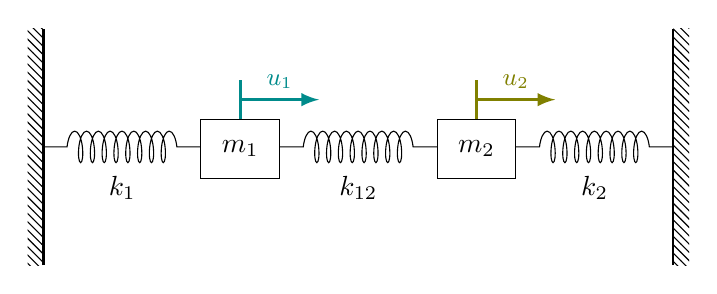
\begin{tikzpicture}
		% left wall
		\fill [pattern = north west lines] (0,0) rectangle ++(.2,3);
		\draw[thick] (.2,0) -- ++(0,3);
		% spring 1
		\draw
		[
		decoration={
			coil,
			aspect=0.3,
			segment length=1.5mm,
			amplitude=2mm,
			pre length=3mm,
			post length=3mm},
		decorate
		] (0.2,1.5) -- ++(2,0)
		node[midway,below=0.25cm,black]{$k_1$};
		% Mass 1
		\node[draw,
		minimum width=1cm,
		minimum height=0.75cm,
		anchor=mid] at (2.7,1.5) {$m_1$};
		% spring 12
		\draw
		[
		decoration={
			coil,
			aspect=0.3,
			segment length=1.5mm,
			amplitude=2mm,
			pre length=3mm,
			post length=3mm},
		decorate
		] (3.2,1.5) -- ++(2,0)
		node[midway,below=0.25cm,black]{$k_{12}$};
		% Mass 2
		\node[draw,
		minimum width=1cm,
		minimum height=0.75cm,
		anchor=mid] at (5.7,1.5) {$m_2$};
		% spring 2
		\draw
		[
		decoration={
			coil,
			aspect=0.3,
			segment length=1.5mm,
			amplitude=2mm,
			pre length=3mm,
			post length=3mm},
		decorate
		] (6.2,1.5) -- ++(2,0)
		node[midway,below=0.25cm,black]{$k_{2}$};
		% right wall
		\fill [pattern = north west lines] (8.2,0) rectangle ++(.2,3);
		\draw[thick] (8.2,0) -- ++(0,3);

		% u1 arrow
		\draw [very thick,
		color1,
		-latex
		] (2.7,1.85) -- ++(0,.5) ++(0,-0.25) -- ++ (1,0)
		node[midway,above]{\small $u_1$};

		% u2 arrow
		\draw [very thick,
		color2,
		-latex
		] (5.7,1.85) -- ++(0,.5) ++(0,-0.25) -- ++ (1,0)
		node[midway,above]{\small $u_2$};
\end{tikzpicture}
\end{document}